\documentclass[a4paper,10pt]{memoir}
\usepackage[italian]{babel}
\usepackage{wrapfig}
\usepackage[pdftex]{graphicx}
\usepackage{graphviz}
\usepackage{amsmath}

\usepackage[chapter]{minted}
\usepackage{adjustbox}
\usepackage{hyperref}
\hypersetup{
  colorlinks   = true,    % Colours links instead of ugly boxes
  urlcolor     = black,    % Colour for external hyperlinks
  linkcolor    = black,    % Colour of internal links
  citecolor    = black      % Colour of citations
}

% import package
\usepackage{FrontespizioSapienza}

\pagestyle{plain}%%to insert the number of the page

% declare info
\FSSTitolo{Titolo}
\FSSFacolta{Ingegneria dell'Informazione, Informatica e Statistica}
\FSSCorso{Informatica}

\FSSCandidato{Edoardo Ottavianelli}
\FSSMatricola{1756005}
\FSSRelatore{Emanuele Panizzi}
\FSSCorrelatore{}
\FSSAnnoAccademico{2019/2020}


\begin{document}

\frontmatter


% print title
\maketitle
\cleardoublepage

%\vspace*{10cm}
%\begin{flushright}
%\textsl{...}
%\end{flushright}
%\cleardoublepage

% ======================================= ABSTRACT ================================================
\begin{abstract}
	abstract
\end{abstract}
\cleardoublepage

\tableofcontents
\cleardoublepage

\mainmatter

\renewcommand\chapterheadstart{}
\renewcommand\printchaptername{}
\renewcommand\chapternamenum{}
\renewcommand\printchapternum{}
\renewcommand\afterchapternum{}
\renewcommand\printchaptertitle[1]{\chaptitlefont \thechapter. \space #1}


% ======================================= CHAPTER 1 ================================================
\chapter{Introduzione a SeismoCloud e obiettivi del progetto}

\section{I terremoti e la loro natura}

\begin{wrapfigure}[14]{r}{0.50\textwidth}
\caption{Composizione della Terra}
\label{fig:crostaterrestre}
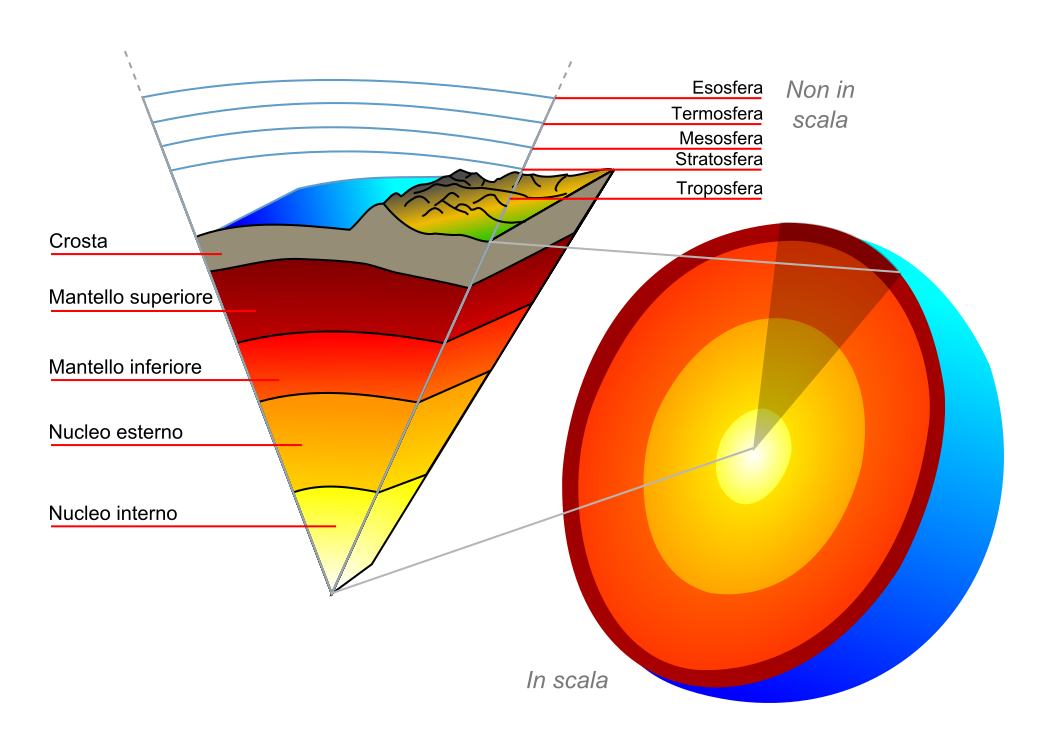
\includegraphics[width=0.50\textwidth]{Chapter-1/crosta-terrestre.png}
\end{wrapfigure}

La terra è composta a strati, o meglio da involucri concentrici (come possiamo notare dalla figura 1.1), ed ognuno di essi ha diverse caratteristiche e particolarità.
Al centro della Terra c'è il \textbf{nucleo interno}, ossia un ammasso viscoso composto quasi esclusivamente da ferro avente un raggio di circa 1250 km. Si raggiungono temperature molto elevate, circa 5000-6000$^{\circ}$C.
A seguire abbiamo il \textbf{nucleo esterno}, principalmente composto per il 20\% da ferro e la restante parte nichel, raggiunge circa i 3000$^{\circ}$C. Comprendendo anche il nucleo interno, ha un raggio di circa 3500 km. \\

Continuando verso l'esterno, troviamo il \textbf{mantello terrestre}, che si divide in superiore ed inferiore.
È composto da diversi metalli ed è difficile stabilire la temperatura dato i moti convettivi del calore, ma si stima intorno ai 500$^{\circ}$C a confine con la crosta terrestre e 3000$^{\circ}$C a confine con il nucleo. \\
Infine abbiamo la \textbf{crosta terrestre}, che partendo dalla superficie, arriva fino a 70 km di profondità. \\
Insieme, il \textit{mantello superiore} e la \textit{crosta terrestre} formano la \textbf{litosfera}.
La litosfera è suddivisa in una decina di placche tettoniche principali e altre numerose placche di minori dimensioni (figura 1.2). Queste placche "galleggiano" sullo strato immediatamente sottostante del mantello superiore. \\
Esse, data la forte pressione e le alte temperature, subiscono sforzi di enormi dimensioni che formano i \textbf{terremoti}. \\
I terremoti sono vibrazioni della crosta terrestre, provocate dallo spostamento  di una o più placche nella litosfera.
Le placche si muovono flettendosi lentamente e poi rilasciando (raggiunto il \textit{punto di rottura}) in maniera elastica tutta l'energia accumulata.
Il punto in cui viene generata questa energia è detto \textbf{ipocentro}, zona in cui sono presenti delle fratture chiamate \textit{faglie}, mentre il punto in superficie posto sulla verticale dell'ipocentro è chiamato \textbf{epicentro}.
\clearpage


\begin{figure}
\centering
\caption{Placche tettoniche}
\label{fig:placchetettoniche}
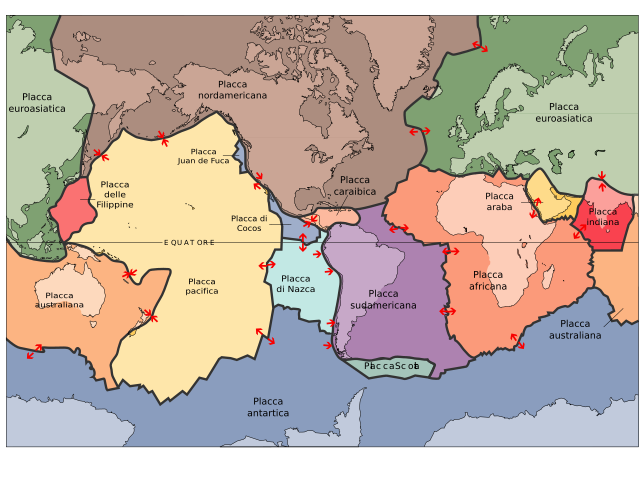
\includegraphics[width=1\textwidth]{Chapter-1/placche-tettoniche.png}
\end{figure}

Esistono tre tipi di faglie: faglie \textit{trascorrenti}, faglie \textit{dirette} e \textit{inverse}.
Esistono in egual numero differenti tipi di onde sismiche. \\
Le \textbf{onde di compressione o longitudinali} fanno comprimere e dilatare la materia nella stessa direzione con cui si propaga l'onda.
Sono anche dette \textit{primarie}, perché sono le onde che viaggiano a velocità più elevate. \\
Le \textbf{onde di taglio o trasversali} fanno compiere alla materia oscillazioni in modo perpendicolare alla loro direzione di propagazione. Hanno effetto solo nei solidi, non possono propagarsi attraverso corpi liquidi o gassosi.
Vengono chiamate anche \textit{onde secondarie}, essendo meno veloci delle precedenti. \\
Le \textbf{onde superficiali}, anche se il nome può essere mal interpretato, non si manifestano in superficie. Questo tipo di onde sono la combinazione delle due precedenti, perciò sono molto complesse e sono le più pericolose. 

\clearpage

\section{Misurazione dei terremoti}

\subsection{Tipologie di terremoti}
Abbiamo 4 differenti tipologie di terremoti: \textit{tettonici}, \textit{vulcanici}, \textit{da crollo} e \textit{artificiali}. \\
I terremoti \textbf{tettonici}, come dice il nome, sono provocati dal movimento delle placche tettoniche e hanno origine lungo le faglie.
Sono i più pericolosi ed i più frequenti. \\
I terremoti \textbf{vulcanici} sono originati dall'attività vulcanica nel sottosuolo. Sono meno pericolosi dei precedenti data la minor energia rilasciata e l'estensione limitata. \\
I terremoti \textbf{da crollo} si originano durante il crollo di montagne, grotte o frane. Hanno una bassa pericolosità e frequenza. \\
Infine, i terremoti \textbf{artificiali} vengono originati da attività umane. Ad esempio, una grande esplosione. In generale, hanno una potenza molto limitata. \\

\subsection{Scale di misurazione}


\clearpage

\section{Utilizzare l'informatica per rilevare terremoti}

placeholder

\clearpage

\section{Piattaforma SeismoCloud}

placeholder

\clearpage

\section{Bisogni della community SeismoCloud}

placeholder

\clearpage

% ======================================= CHAPTER 2 ================================================
\chapter{Architettura di Node-RED adattata a SeismoCloud}

\section{Perché Node-RED}

placeholder

\clearpage

\section{Difficoltà e limiti nell'uso di Node-RED}

placeholder

\clearpage

\section{Pianificazione del progetto}

placeholder

\clearpage

\section{Architettura adattata a SeismoCloud}

placeholder

\clearpage

\section{Implementazione delle funzionalità tramite nodi}

placeholder

\clearpage

\section{Ottimizzazione delle prestazioni}

placeholder

\clearpage

% ======================================= CHAPTER 3 ================================================
\chapter{Sicurezza e protezione dei dati}

\section{Sicurezza nella piattaforma Node-RED}

placeholder

\clearpage

\section{Ricerca ed analisi di vulnerabilità}

placeholder

\clearpage

\section{Risoluzione dei problemi}

placeholder

\clearpage


% ======================================= CHAPTER 4 ================================================
\chapter{Test, conclusioni e sviluppi futuri}

\section{Iterazioni dei Test}

placeholder

\clearpage

\section{Conclusioni}

placeholder

\clearpage

\section{Sviluppi futuri}

placeholder

\clearpage

\refstepcounter{chapter}

\chapter*{Ringraziamenti}

\cleardoublepage

\refstepcounter{chapter}

% ======================================= BIBLIOGRAPHY ================================================
\begin{thebibliography}{9}

\bibitem{placeholder}
	\textbf{placeholder}.
	placeholder

\end{thebibliography}

\end{document}